%%%%%%%%%%%%%%%%%%%%%%%%%%%%%%%%%%%%%%%%%
% Beamer Presentation
% LaTeX Template
% Version 1.0 (10/11/12)
%
% This template has been downloaded from:
% http://www.LaTeXTemplates.com
%
% License:
% CC BY-NC-SA 3.0 (http://creativecommons.org/licenses/by-nc-sa/3.0/)
%
%%%%%%%%%%%%%%%%%%%%%%%%%%%%%%%%%%%%%%%%%

%----------------------------------------------------------------------------------------
%   PACKAGES AND THEMES
%----------------------------------------------------------------------------------------

\documentclass{beamer}

\mode<presentation> {

% The Beamer class comes with a number of default slide themes
% which change the colors and layouts of slides. Below this is a list
% of all the themes, uncomment each in turn to see what they look like.

%\usetheme{default}
%\usetheme{AnnArbor}
%\usetheme{Antibes}
%\usetheme{Bergen}
%\usetheme{Berkeley}
%\usetheme{Berlin}
%\usetheme{Boadilla}
%\usetheme{CambridgeUS}
%\usetheme{Copenhagen}
%\usetheme{Darmstadt}
%\usetheme{Dresden}
%\usetheme{Frankfurt}
%\usetheme{Goettingen}
%\usetheme{Hannover}
%\usetheme{Ilmenau}
%\usetheme{JuanLesPins}
%\usetheme{Luebeck}
\usetheme{Madrid}
%\usetheme{Malmoe}
%\usetheme{Marburg}
%\usetheme{Montpellier}
%\usetheme{PaloAlto}
%\usetheme{Pittsburgh}
%\usetheme{Rochester}
%\usetheme{Singapore}
%\usetheme{Szeged}
%\usetheme{Warsaw}

% As well as themes, the Beamer class has a number of color themes
% for any slide theme. Uncomment each of these in turn to see how it
% changes the colors of your current slide theme.

%\usecolortheme{albatross}
%\usecolortheme{beaver}
%\usecolortheme{beetle}
%\usecolortheme{crane}
%\usecolortheme{dolphin}
%\usecolortheme{dove}
%\usecolortheme{fly}
%\usecolortheme{lily}
%\usecolortheme{orchid}
%\usecolortheme{rose}
%\usecolortheme{seagull}
%\usecolortheme{seahorse}
%\usecolortheme{whale}
%\usecolortheme{wolverine}

%\setbeamertemplate{footline} % To remove the footer line in all slides uncomment this line
%\setbeamertemplate{footline}[page number] % To replace the footer line in all slides with a simple slide count uncomment this line

%\setbeamertemplate{navigation symbols}{} % To remove the navigation symbols from the bottom of all slides uncomment this line
}

\usepackage{graphicx} % Allows including images
\usepackage{grffile}
\usepackage{booktabs} % Allows the use of \toprule, \midrule and \bottomrule in tables
\usepackage[utf8]{inputenc}
\usepackage{amsmath}
\usepackage{amsfonts}
\usepackage{amssymb}
\usepackage{tabto}
\usepackage{braket}

\newcommand{\tabs}[2]{\hspace*{7pt}\makebox[0pt][c]{#1}\hspace*{35pt}\makebox[0pt][c]{#2}}

\begin{document}

%\begin{frame}
%\titlepage % Print the title page as the first slide
%\end{frame}

%----------------------------------------------------------------------------------------
%   PRESENTATION SLIDES
%----------------------------------------------------------------------------------------

\begin{frame}{Wigner distribution}
	\begin{itemize}
		\vfill
		\item General definition: if $\rho = \sum_i p_i \ket{\psi_i}\mkern-4mu\bra{\psi_i}$, then the Wigner distribution is:
		$$ W(x,p) = \frac{1}{\pi} \sum_i p_i \int dy\,\psi^*_i(x+y) \psi(x-y) e^{2ipy} $$
		\vfill
		\item It is real valued and maps the wave function to phase space. The following holds:
		$$ |\psi(x)|^2 = \int dp\, W(x,p),$$
		$$ |\psi(p)|^2 = \int dx\, W(x,p),$$
		$$ <G(x,p)> = \int dx\, \int dp\, W(x,p)G(x,p).$$
		\vfill
		\item However it can also take negative values and in quantum mechanics you cannot say there is a probability to have some $x$ and $p$ values at the same time.
		\vfill
	\end{itemize}
\end{frame}

\begin{frame}{Wigner distribution}
	\begin{itemize}
		\vfill
		\item Wavefunction represented using a basis of Legendre functions.
		\vfill
		\item Wavefunction sampled on a uniform grid and the transformation done using FFTW.
		\vfill
		\item Wigner distribution of two Gaussian wavefunctions $\psi(x) = \frac{1}{\sqrt[4]{\pi\sigma^2}}e^{-\frac{x^2}{2\sigma^2}}$, with $\sigma=1$ and $\sigma=2$:\\
		\begin{minipage}[t][][b]{0.49\linewidth}
			\centering
			\vspace*{-5pt}
			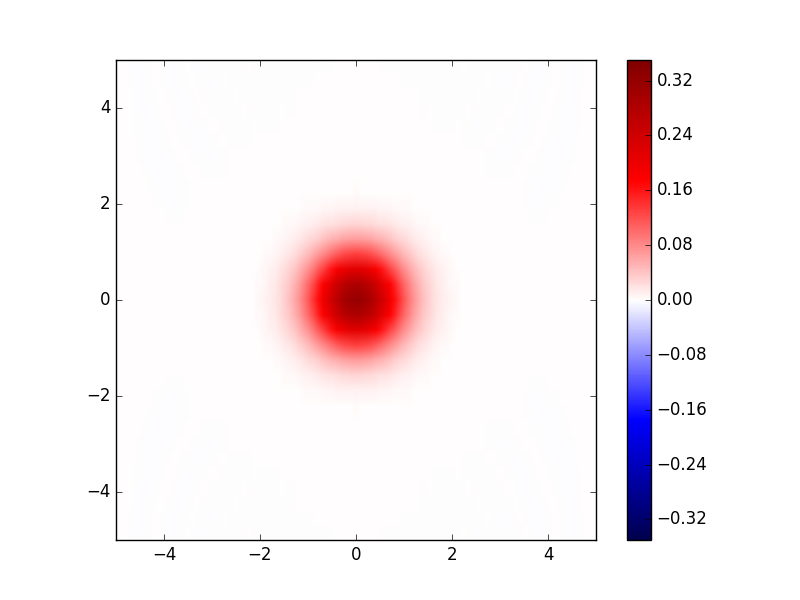
\includegraphics[width=1\linewidth]{test0}
		\end{minipage}
		\begin{minipage}[t][][b]{0.49\linewidth}
			\centering
			\vspace*{-5pt}
			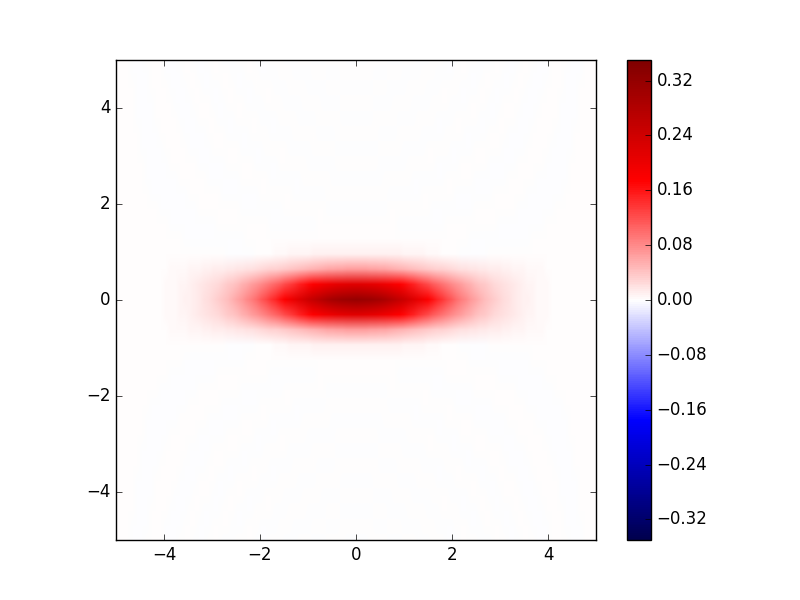
\includegraphics[width=1\linewidth]{test1}
		\end{minipage}
		\vfill
	\end{itemize}
\end{frame}

\begin{frame}{Harmonic oscillator}
	\begin{itemize}
		\vfill
		\item For a harmonic potential the Wigner distribution behaves classically. Each point just moves as if a classical particle with that momentum and location.
		\vfill
		\item Wigner distribution of the first two ground states of the harmonic oscillator $\psi_1(x) = \frac{1}{\sqrt[4]\pi}e^{-x^2}$, \kern4em $\psi_2(x) = \frac{\sqrt{2}x}{\sqrt[4]\pi}e^{-x^2}$:
		\begin{minipage}[t][][b]{0.49\linewidth}
			\centering
			\vspace*{-5pt}
			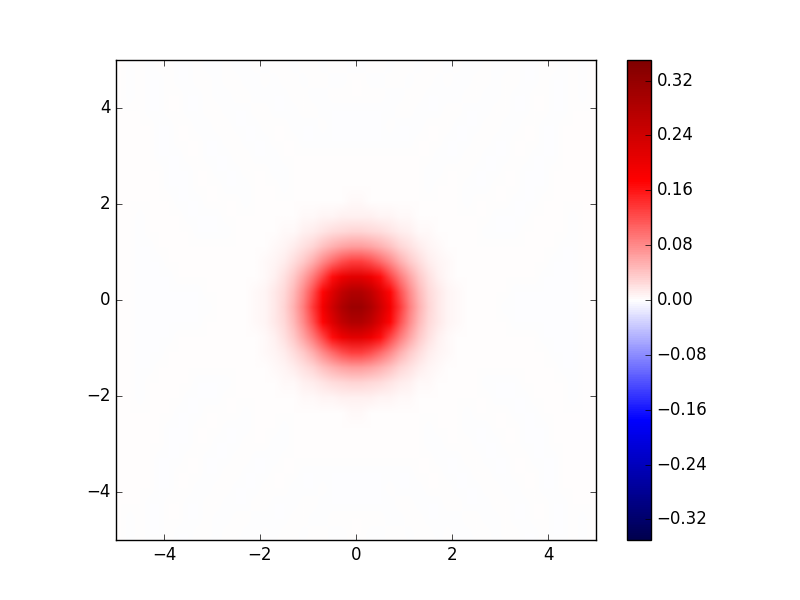
\includegraphics[width=1\linewidth]{oscEigen0}
		\end{minipage}
		\begin{minipage}[t][][b]{0.49\linewidth}
			\centering
			\vspace*{-5pt}
			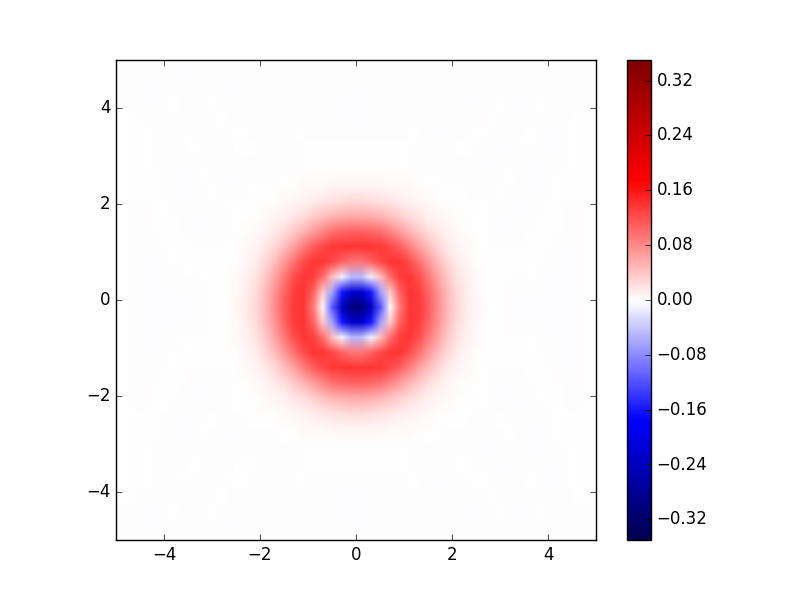
\includegraphics[width=1\linewidth]{oscEigen1}
		\end{minipage}
		\vfill
		\item We notice negative values of the distribution.
		\vfill
	\end{itemize}
\end{frame}

\begin{frame}{Coherent states}
	\begin{itemize}
		\vfill
		\item For a coherent state the graph of $|\psi(x)|^2$ oscillates back and forth as a classical particle.
		\vfill
		\item Coherent state is characterized by a complex number $\alpha$. The real and imaginary values of which give the $x$ and $p$ displacement of the Gaussian Wigner distribution. An example for $\alpha = 1+i$:
		\begin{minipage}[t][][b]{\linewidth}
			\centering
			\vspace*{-10pt}
			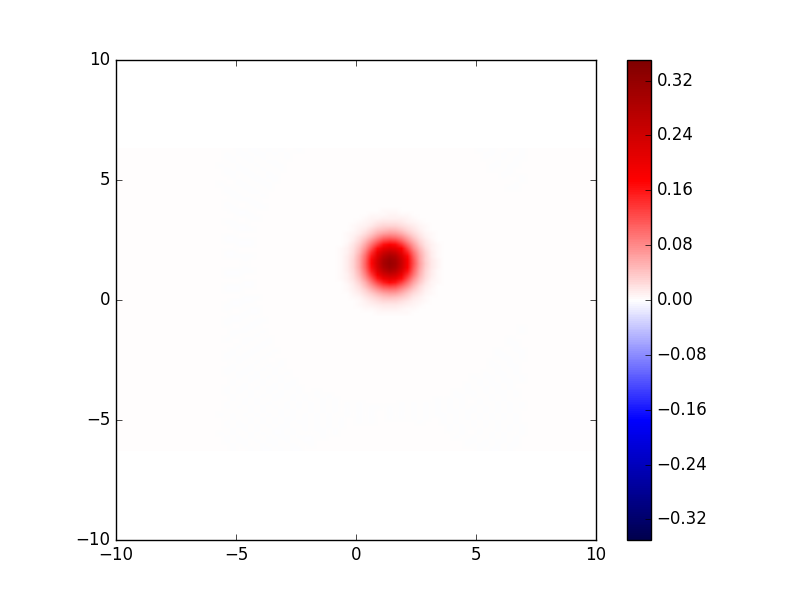
\includegraphics[width=0.6\linewidth]{oscCoh11}
		\end{minipage}
		\vfill
	\end{itemize}
\end{frame}


\begin{frame}{Pure and mixed states}
	\begin{itemize}
		\vfill
		\item Here I plot the pure and mixed states of two coherent states of the harmonic oscillator:\\
		\begin{minipage}[t][][b]{0.49\linewidth}
			\centering
			\vspace*{-5pt}
			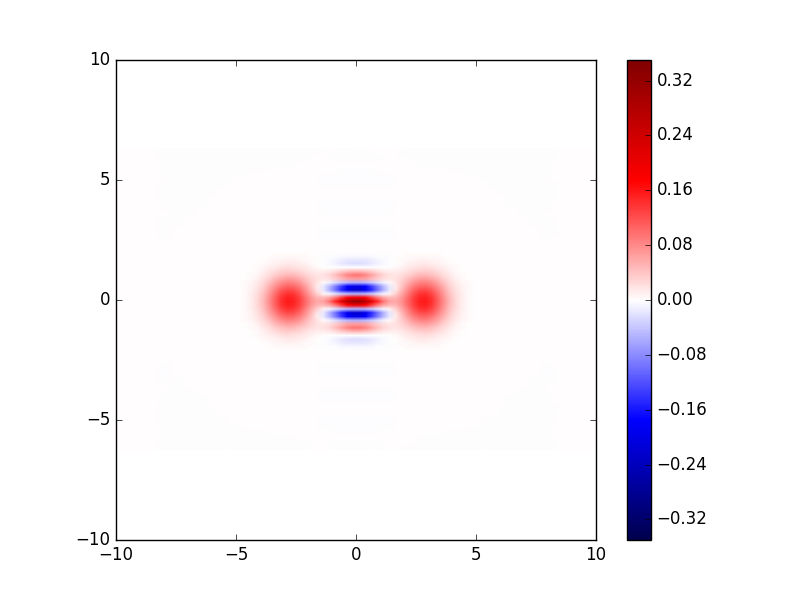
\includegraphics[width=1\linewidth]{oscPure}
		\end{minipage}
		\begin{minipage}[t][][b]{0.49\linewidth}
			\centering
			\vspace*{-5pt}
			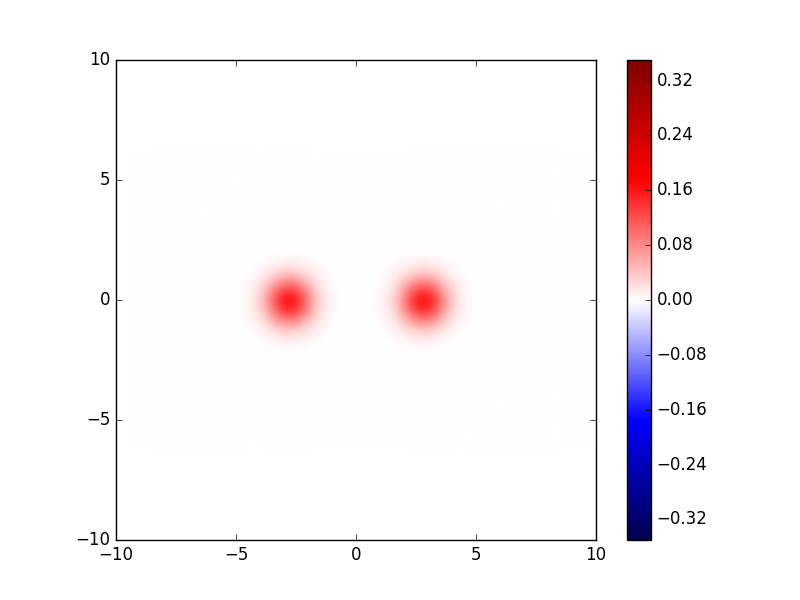
\includegraphics[width=1\linewidth]{oscMixed}
		\end{minipage}
		\vfill
		\item The pure state has extra interference terms.
		\vfill
	\end{itemize}
\end{frame}

\begin{frame}{Time evolution}
	\begin{itemize}
		\vfill
		\item Time evolution simulations.
		\vfill
	\end{itemize}
\end{frame}

	
\end{document}